\documentclass{../../slides-style}

\slidetitle{Юнит-тестирование и системы сборки}{03.10.2026}

\begin{document}

    \begin{frame}[plain]
        \titlepage
    \end{frame}

    \section{Системы сборки}

    \begin{frame}{Системы сборки}
        \begin{outline}
            \1 Нужны, чтобы сборка не зависела от среды разработки
                \2 Воспроизводимость сборки
                \2 \enquote{Пакетный режим}, CI
            \1 Умеют вычислять зависимости между компонентами, управлять внешними зависимостями
                \2 И автоматически скачивать нужные пакеты при сборке
            \1 Не только, собственно, сборка: тестирование, создание документации, инсталляторов, отчётов и т.д.
            \1 Maven
            \1 Gradle
        \end{outline}
    \end{frame}

    \subsection{Maven}

    \begin{frame}{Maven, основные принципы}
        \begin{outline}
            \1 Декларативность
            \1 Convention Over Configuration
                \2 Стандартная структура папок
            \1 Плагины
            \1 Project Object Model
            \1 Жизненный цикл
            \1 Координаты
                \2 groupId
                \2 artifactId
                \2 version
            \1 Репозиторий и on-demand-скачивание пакетов
                \2 СИстема поиска пакетов --- \url{https://mvnrepository.com/}
                \2 Локальный кеш: ~/.m2/repository
        \end{outline}
    \end{frame}

    \begin{frame}{Maven, стандартная структура папок}
        \begin{outline}
            \1 pom.xml
            \1 src
                \2 main
                    \3 java
                    \3 resources
                \2 test
                    \3 java
                    \3 resources
            \1 target
        \end{outline}
    \end{frame}

    \subsection{Gradle}

    \begin{frame}{Gradle}
        \begin{outline}
            \1 Более легковесный и современный, чем Maven
            \1 Декларативный предметно-ориентированный язык на основе Groovy или Kotlin
            \1 Использует Convention Over Configuration, но легко переопределить
                \2 Та же структура папок по умолчанию
            \1 Использует репозиторий Maven для динамической загрузки зависимостей
            \1 build.gradle, settings.gradle
            \1 gradle-wrapper
                \2 gradlew, gradlew.bat
                \2 gradle-wrapper.jar, gradle-wrapper.properties
        \end{outline}
    \end{frame}

    \section{Юнит-тестирование}

    \begin{frame}{Модульное тестирование, информация к размышлению}
        \begin{outline}
            \1 Программа из сотни строк может иметь $10^{18}$ путей исполнения
                \2 Полный перебор занял бы слишком много времени, а в реальных программах путей исполнения ещё больше
            \1 После передачи на тестирование в программах в среднем от 1 до 3 ошибок на 100 строк кода
            \1 В процессе разработки --- 1.5 ошибок на 1 строку кода (!)
            \1 Если для исправления ошибки надо изменить не более 10 операторов, с первого раза это делают правильно в 50\% случаев
            \1 Если для исправления ошибки надо изменить не более 50 операторов, с первого раза это делают правильно в 20\% случаев
        \end{outline}
    \end{frame}

    \begin{frame}{JUnit 6}
        \begin{outline}
            \1 JUnit --- самая известная библиотека юнит-тестирования для Java
            \1 JUnit 6 --- его последняя версия (часто до сих пор используется JUnit 5 или даже 4)
            \1 Отлично интегрируется с IDE
                \2 Генерация заглушек тестов, запуск тестов прямо из редактора и т.д.
                \2 Справедливости ради, тесты хорошо пишутся LLMками, так что это не так важно
            \1 Тест --- это отдельный класс, в котором есть методы, помеченные аннотацией \mintinline{java}|@Test|
            \1 Внутри теста обычно три фазы
                \2 Настройка тестового окружения
                \2 Выполнение действия, которое хотим тестировать
                \2 Проверка результатов
                    \3 Вызовы assertEquals, assertNull, assertTrue и т.д.
        \end{outline}
    \end{frame}

    % \begin{frame}{Демонстрация}
    %     \begin{center}
    %         \huge{Демонстрация}
    %     \end{center}
    % \end{frame}

    \begin{frame}{Ещё аннотации}
        \begin{outline}
            \1 \mintinline{java}|@BeforeEach| --- метод, запускающийся перед каждым тестом
            \1 \mintinline{java}|@AfterEach| --- метод, запускающийся после каждого теста
            \1 \mintinline{java}|@BeforeAll| --- метод, запускающийся перед всеми тестами в классе (должен быть static)
            \1 \mintinline{java}|@AfterAll| --- метод, запускающийся после всех тестов в классе (должен быть static)
            \1 \mintinline{java}|@Disabled| --- тест отключён и не запускается
        \end{outline}
    \end{frame}

    \begin{frame}{Assertions}
        \framesubtitle{Наиболее интересные}
        \begin{outline}
            \1 assertEquals
                \2 Обратите внимание на порядок параметров, сначала ожидаемое, затем то, что получилось
            \1 assertArrayEquals
            \1 assertTrue/assertFalse
            \1 assertNull/assertNotNull
            \1 assertThrows
            \1 fail
        \end{outline}
    \end{frame}

    \begin{frame}{Best practices}
        \begin{outline}
            \1 Независимость тестов
                \2 Желательно, чтобы поломка одного куска функциональности ломала один тест
            \1 Тесты должны работать быстро
                \2 И запускаться после каждой сборки
                    \3 Continuous Integration
            \1 Тестов должно быть много
                \2 Следите за Code coverage, это хороший индикатор непокрытого и мёртвого кода
            \1 Каждый тест должен проверять конкретный тестовый сценарий
                \2 Нельзя ловить исключения в тесте без крайней нужды
                \2 С большой осторожностью пользоваться Random-ом
            \1 Именование тестов: \url{http://stackoverflow.com/questions/155436/unit-test-naming-best-practices}
            \1 Test-driven development
        \end{outline}
    \end{frame}

    \section{Библиотеки для написания assert-ов}

    \begin{frame}{Hamcrest}
        \begin{outline}
            \1 Библиотека матчеров --- объектов, представляющих логическое условие
            \1 Нужна прежде всего для удобства записи assert-ов в модульных тестах
                \2 И для читаемости, что немаловажно
            \1 В JUnit 4 входила в зависимости фреймворка, дальше --- надо добавлять отдельно
        \end{outline}
    \end{frame}

    \begin{frame}[fragile]{Hamcrest, пример}
        \begin{outline}
            \1 \mintinline{java}|assertThat(someString, is(not(equalTo(someOtherString))));|
            \1 \mintinline{java}|assertThat(list, everyItem(greaterThan(1)));|
            \1 \mintinline{java}|assertThat(cat.getKittens(), hasItem(someKitten));|
            \1 \mintinline{java}|assertThat("test", anyOf(is("testing"), containsString("est")));|
            \1 
                \begin{minted}{java}
assertThat(x, 
    allOf(greaterThan(0), lessThanOrEqualTo(10)));
                \end{minted}
        \end{outline}
    \end{frame}

    \begin{frame}[fragile]{AssertJ}
        \begin{outline}
            \1 Библиотека fluent assertions --- ещё более человекочитаемый синтаксис, чем Hamcrest
            \1 Пример (из документации):
                \begin{footnotesize}
                    \begin{minted}{java}
assertThat(frodo.getName()).isEqualTo("Frodo");
assertThat(frodo).isNotEqualTo(sauron);

assertThat(frodo.getName()).startsWith("Fro")
    .endsWith("do")
    .isEqualToIgnoringCase("frodo");

assertThat(fellowshipOfTheRing)
    .hasSize(9)
    .contains(frodo, sam)
    .doesNotContain(sauron);

assertThatThrownBy(() -> 
    { throw new Exception("boom!"); }).hasMessage("boom!");
                    \end{minted}
                \end{footnotesize}
        \end{outline}
    \end{frame}

    \begin{frame}[fragile]{Truth}
        \begin{outline}
            \1 Библиотека fluent assertions от Google, альтернатива AssertJ
                \2 Схожая философия, Truth более простой (что может быть как плюсом, так и минусом)
            \1 Пример (из документации):
                \begin{minted}{java}
assertThat(projectsByTeam())
    .valuesForKey("corelibs")
    .containsExactly("guava", "dagger", "truth", "auto", "caliper");
                \end{minted}
        \end{outline}
    \end{frame}

    \section{Mock-объекты}

    \begin{frame}{Mock-объекты}
        \begin{outline}
            \1 Объекты-заглушки, симулирующие поведение реальных объектов и контролирующие обращения к своим методам
                \2 Как правило, такие объекты создаются с помощью библиотек
            \1 Используются, когда реальные объекты использовать
                \2 Слишком долго
                \2 Слишком опасно
                \2 Слишком трудно
                \2 Для добавления детерминизма в тестовый сценарий
                \2 Пока реального объекта ещё нет
                \2 Для изоляции тестируемого объекта
            \1 Для использования mock-объекта требуется какой-то механизм внедрения объекта
                \2 Как правило, как параметр конструктора или через поле
        \end{outline}
    \end{frame}

    \begin{frame}{Объекты-заглушки}
        \begin{center}
            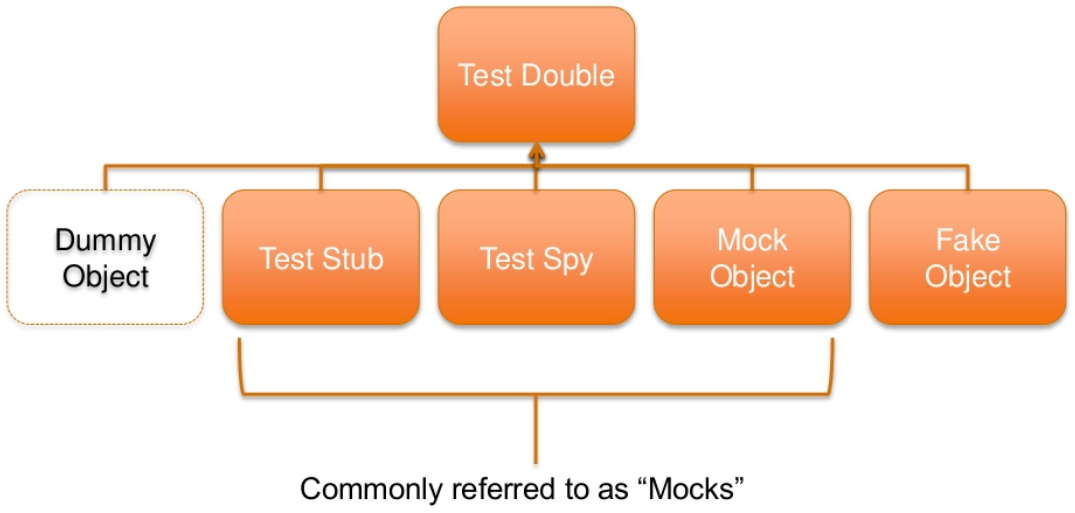
\includegraphics[width=0.9\textwidth]{testDoubles.png}
        \end{center}
    \end{frame}

    \begin{frame}{Stubs}
        \begin{outline}
            \1 Захардкоженные объекты, реализующие нужный интерфейс
            \1 Наивная или вообще отсутствующая реализация
                \2 Возможно какие-то assert’ы или полезная логика для теста
        \end{outline}
        \begin{center}
            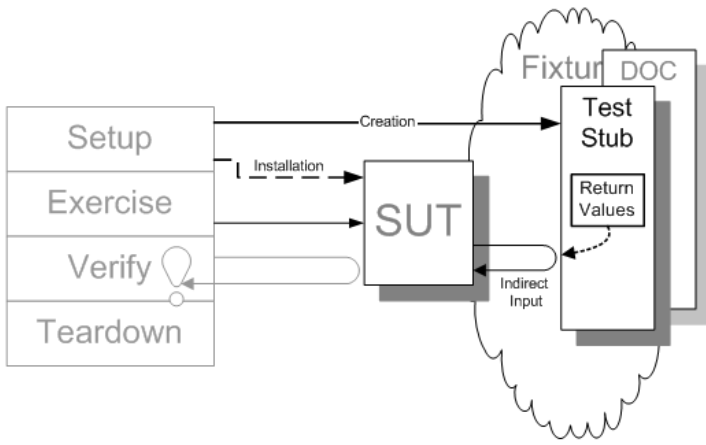
\includegraphics[width=0.6\textwidth]{stub.png}
            \attribution{http://xunitpatterns.com}
        \end{center}
    \end{frame}

    \begin{frame}{Spies}
        \begin{outline}
            \1 Запуск теста, затем проверка условий и ограничений
        \end{outline}
        \begin{center}
            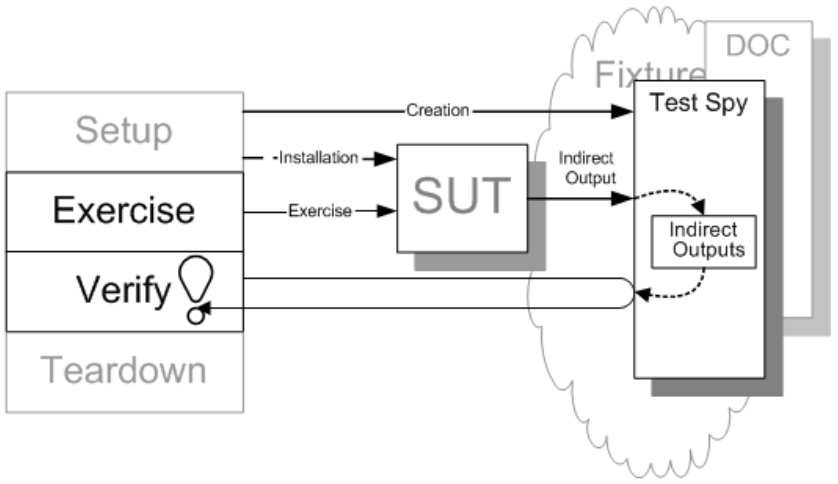
\includegraphics[width=0.6\textwidth]{spy.png}
            \attribution{http://xunitpatterns.com}
        \end{center}
    \end{frame}

    \begin{frame}{Mocks}
        \begin{outline}
            \1 Конфигурирование объекта перед запуском теста
        \end{outline}
        \begin{center}
            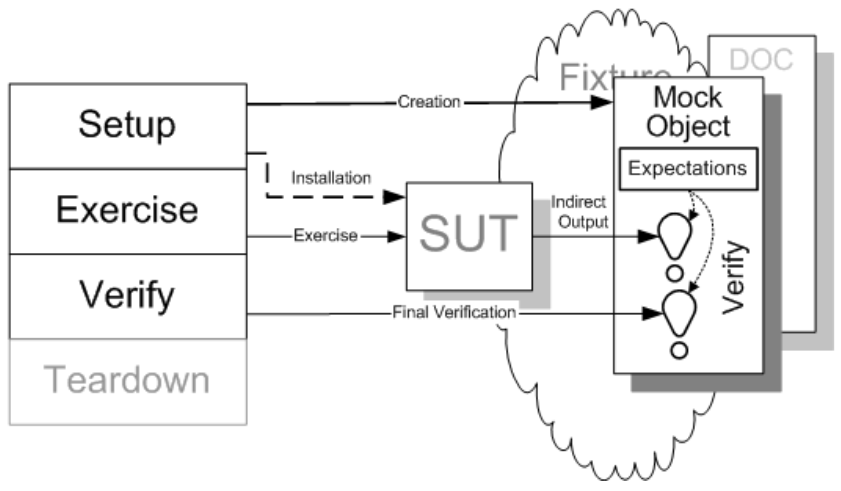
\includegraphics[width=0.6\textwidth]{mock.png}
            \attribution{http://xunitpatterns.com}
        \end{center}
    \end{frame}

    \begin{frame}{Mockito}
        \begin{outline}
            \1 Один из самых известных фреймворков для мок-объектов
                \2 Но далеко не единственный
            \1 \url{http://site.mockito.org/}
            \1 \url{https://github.com/mockito/mockito}
        \end{outline}
    \end{frame}

    \begin{frame}[fragile]{Классический тест}
        \begin{minted}{java}
@Test 
public void test() throws Exception {
    // Arrange
    var testee = new UnitToTest();
    var helper = new Helper();
    // Act
    testee.doSomething(helper);
    // Assert
    assertTrue(helper.somethingHappened());
}
        \end{minted}
    \end{frame}

    \begin{frame}[fragile]{Тест с mock-объектом}
        \begin{minted}{java}
@Test
public void test() throws Exception {
    // Arrange, prepare behaviour
    Helper aMock = mock(Helper.class);
    when(aMock.isCalled()).thenReturn(true);
    // Act
    testee.doSomething(aMock);
    // Assert - verify interactions (optional)
    verify(aMock).isCalled();
}
        \end{minted}
    \end{frame}

    \begin{frame}[fragile]{Создание mock-объектов}
        \begin{outline}
            \1 \mintinline{java}|IMyClass myMock = mock(IMyClass.class)|
            \1 \mintinline{java}|MyClass myMock = mock(MyClass.class)|
            \1 \mintinline{java}|@Mock private MyClass myMock;|
                \2 
                    \begin{minted}{java}
@Before public void setup() { 
    MockitoAnnotations.openMocks(this); 
}
                    \end{minted}
        \end{outline}
    \end{frame}

    \begin{frame}[fragile]{when(...)}
        \begin{outline}
            \1 \mintinline{java}|when(mock.someMethod()).thenReturn(10);|
            \1 
                \begin{minted}{java}
when(mock.someMethod("some arg"))
    .thenThrow(new RuntimeException());
                \end{minted}
            \1 \mintinline{java}|when(mock.someMethod(anyString())).thenReturn(42);|
            \1 \mintinline{java}|when(mock.someMethod(anyInt())).thenReturn("element");|
            \1 
                \begin{minted}{java}
when(mock.someMethod(argThat(list -> list.size() < 3)))
    .thenReturn(null);
                \end{minted}
        \end{outline}
    \end{frame}

    \begin{frame}[fragile]{Последовательные вызовы}
        \begin{outline}
            \1 
                \begin{minted}{java}
when(mock.someMethod("some arg"))
    .thenThrow(new RuntimeException())
    .thenReturn("foo");
                \end{minted}
            \1 
                \begin{minted}{java}
when(mock.someMethod("some arg"))
    .thenReturn("one", "two", "three");
                \end{minted}
            \1 Но:
                \begin{minted}{java}
when(mock.someMethod("some arg")).thenReturn("one")
when(mock.someMethod("some arg")).thenReturn("two")
                \end{minted}
        \end{outline}
    \end{frame}

    \begin{frame}[fragile]{Подмена действия}
        \begin{minted}{java}
when(mock.someMethod(anyString())).thenAnswer(new Answer() {
     Object answer(InvocationOnMock invocation) {
         Object[] args = invocation.getArguments();
         return "called with arguments: " + Arrays.toString(args);
     }
 });
 
 //the following prints "called with arguments: [foo]"
 System.out.println(mock.someMethod("foo"));
        \end{minted}
    \end{frame}

    \begin{frame}[fragile]{verify(...)}
        \begin{outline}
            \1 \mintinline{java}|verify(mock).someMethod();|
            \1 \mintinline{java}|verify(mock, timeout(100)).someMethod();|
            \1 
                \begin{minted}{java}
verify(mock).someMethod(
    anyInt(), anyString(), eq("third argument"));
                \end{minted}
            \1 
                \begin{minted}{java}
verify(mock).someMethod(
    argThat(someString -> someString.length() > 5));
                \end{minted}
        \end{outline}
    \end{frame}

    \begin{frame}[fragile]{Повторные вызовы}
        \begin{outline}
            \1 \mintinline{java}|verify(mock, times(2)).someMethod();|
            \1 \mintinline{java}|verify(mock, never()).someMethod();|
                \2 \mintinline{java}|verifyNoInteractions(mockTwo);|
            \1 \mintinline{java}|verify(mock, atLeastOnce()).someMethod();|
            \1 \mintinline{java}|verify(mock, atLeast(2)).someMethod();|
            \1 \mintinline{java}|verify(mock, atMost(5)).someMethod();|
            \1 
                \begin{minted}{java}
InOrder inOrder = inOrder(mock);
inOrder.verify(mock).someMethod("was called first");
inOrder.verify(mock).someMethod("was called second");
                \end{minted}
        \end{outline}
    \end{frame}

    \begin{frame}[fragile]{spy(...)}
        \begin{small}
            \begin{minted}{java}
List list = new LinkedList();
List spy = spy(list);

when(spy.size()).thenReturn(100);

spy.add("one");
spy.add("two");

//prints "one" - the first element of a list
System.out.println(spy.get(0));

//size() method was stubbed - 100 is printed
System.out.println(spy.size());

verify(spy).add("one");
verify(spy).add("two");
            \end{minted}
        \end{small}
    \end{frame}

    \begin{frame}{Примерное соотношение объёма тестов в проекте}
        \begin{center}
            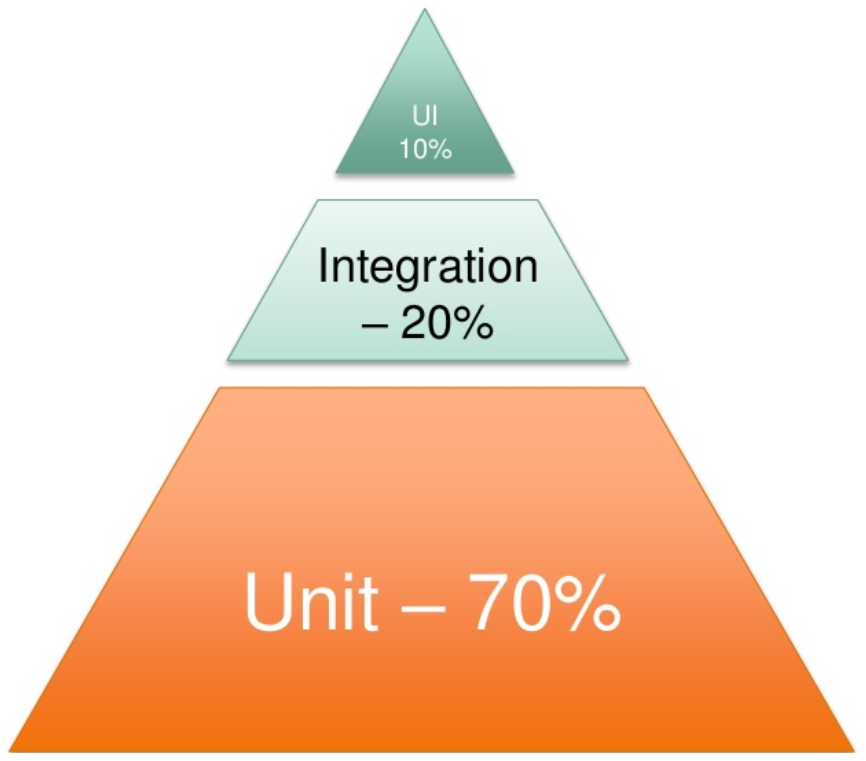
\includegraphics[width=0.6\textwidth]{testPyramid.png}
        \end{center}
    \end{frame}

    \section{Задание}

    \begin{frame}{Задание на остаток пары}
        \begin{outline}
             \1 Поделиться на команды по 2-3 человека
             \1 Написать модульные тесты на StringSet и List с предыдущей пары
             \1 Используйте JUnit, одну из библиотек матчеров на выбор и Mockito
                \2 Mockito для изоляции тестов на хеш-таблицу, чтобы они не зависели от списка
            \1 Используйте правильное именование тестов и подход \enquote{Arrange-Act-Assert}
        \end{outline}
    \end{frame}

\end{document}
